\documentclass{article}

\usepackage[english]{babel}
\usepackage[letterpaper, top=2cm, bottom=2cm, left=3cm, right=3cm, marginparwidth=1.75cm]{geometry}
\usepackage{amsmath}
\usepackage{graphicx}
\usepackage[colorlinks=true, allcolors=blue]{hyperref}
\geometry{a4paper, total={170mm,257mm}, left=20mm, top=20mm}

\pagenumbering{arabic}

\begin{document}

\begin{titlepage}
    \begin{center}
        \vspace*{1cm}
            
        \Huge
        \textbf{Simulation of Ising model}
            
        \vspace{4cm}
        \Large  
        \textbf{Rithik Rai}\\  
        \textbf{3rd Semester MSc Physics}\\
        \textbf{Registration Number: 31822026}\\
        \vspace{4cm}
        Presented to,\\
        \textbf{Dr. Sasidevan V}\\
        Assistant Professor,\\
        Department of Physics\\
        Cochin University of Science and Technology\\
        November 25, 2023.
            
    \end{center}
\end{titlepage}

\section{Objective}

To simulate the 2D ferromagnetic Ising model on a square lattice and investigate:
\begin{itemize}
    \item Phase transition point
    \item Average magnetization as a function of temperature
    \item Magnetic susceptibility as a function of temperature
    \item Specific heat as a function of temperature
\end{itemize}

\section{Theoretical Background}
\textbf{Understanding the Ising Model}

The Ising model is a mathematical representation designed to explore phase transitions in magnetic systems, particularly in ferromagnetic materials. It operates on a lattice, a finite set of points in dimension D. Each lattice site can assume one of two 'spin' states: +1 or -1. The former corresponds to spin-up, and the latter to spin-down. Denoting N lattice sites as $S_{i}$, where $i = 1, 2, 3, \ldots, N$, the spins only interact with their nearest neighbors. Utilizing periodic boundary conditions ensures each spin has an equal number of nearby spins, even at the lattice edges.

The Hamiltonian describing the system's energy with a spin configuration is given by:

\[H=-\sum_{<ij> }J_{ij}\sigma _{i}\sigma _{j} - B\sum_{i}\sigma _{i}\]

where $J_{ij}$ represents the exchange energy between spins $\sigma _{i}$ and $\sigma _{j}$, and B is the applied magnetic field. In the absence of an external magnetic field, the Hamiltonian reduces to:

\[H=-\sum_{<ij> }J_{ij}\sigma _{i}\sigma _{j}\]

For ferromagnetic materials, J takes a positive value.

\section{Phase Transitions in Ferromagnetic Systems}
The Ising model sheds light on phase transitions in ferromagnetic systems. At low temperatures, thermal energy diminishes, making spin interaction energy more dominant. Spins tend to align parallelly, forming a ferromagnetic phase to minimize energy. Conversely, at high temperatures, thermal fluctuations disrupt spin alignment, resulting in a disordered paramagnetic phase with randomly oriented spins. The transition between these states is the Curie point or critical point, marked by the Curie temperature ($T_{c}$). Below $T_{c}$, magnetization (M) exhibits a non-zero value, dropping abruptly to zero at $T_{c}$. Quantities like magnetic susceptibility and specific heat describe this phase change near $T_{c}$.

\section{Observable Quantities from Simulation}
The simulation aims to extract observables: average energy (E), average magnetization (M), specific heat ($C_{v}$), and magnetic susceptibility ($\chi$), given by:
\[\left \langle E \right \rangle= \frac{1}{2}\left \langle \sum_{i,j}H_{_{ij}}^{} \right \rangle\]
\[ \left \langle M \right \rangle=\frac{1}{N^{2}}\sum_{i,j}\sigma_{i,j} ^{}\]
\[C_{v}=\frac{\beta }{T}\left ( \left \langle E^{2} \right \rangle -\left \langle E \right \rangle^{2}\right)\]
\[ \chi =\beta\left ( \left \langle M^{2} \right \rangle -\left \langle M \right \rangle^{2}\right)\]
where $\beta = \frac{1}{k_{b}T}$, with $k_{b}$ as the Boltzmann constant. A sudden drop of magnetization to zero at $T_{c}$ signifies a phase transition.

\section{Simulation Procedure}
We employ the Metropolis Algorithm, a standard method for generating sample configurations of the Ising model in thermal equilibrium at a specific temperature.
\begin{itemize}
    \item A 2D NxN matrix is created, where each lattice site can be +1 or -1.
    \item For periodic boundary conditions, we use the modulo operator, taking neighboring sites as $((i + 1) \mod (N), j)$ instead of $((i + 1), j)$.
    \item A lattice site is randomly selected, and $\triangle E = (E_{\text{final}} - E_{\text{initial}})$ is calculated for a fixed temperature.
    \item If $\triangle E \leq 0$, the spin flips because the change is favorable (i.e., the final state has lower energy).
    \item If $\triangle E > 0$, a random number $x$ is generated on the interval [0, 1]. The spin flips only if ${e^{-\triangle E/k_{b}T} > x}$ (i.e., the particle has enough energy to flip the spin), otherwise, the spin change is rejected.
    \item This process is repeated, and the modified state of the system at a particular temperature T, represented by a new matrix, is returned.
    \item The procedure is repeated at different temperatures, noting the energy and magnetization for each step.
\end{itemize}

Onsager's solution for the critical temperature for a square lattice is:
\[T_{c} = \frac{2}{\log(1 + \sqrt{2})} = 2.269 J/k_{B}\]
where J = 1.

\section{Results}

\begin{figure}[h]
    \centering
    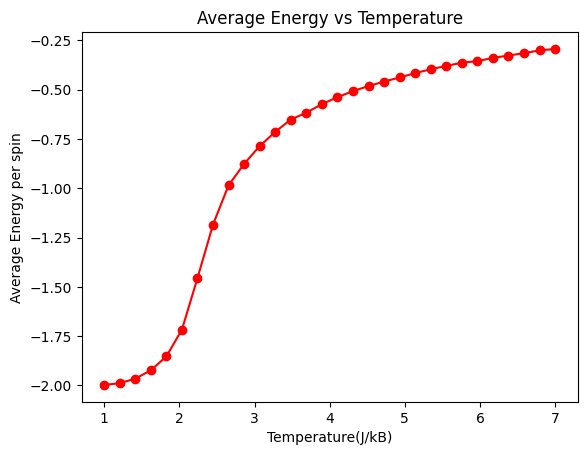
\includegraphics[scale=0.8]{avgenergyvstemp.png}
    \caption{\textbf{Average energy as a function of temperature}}
    \label{fig:avg_energy_vs_temp}
\end{figure}

\begin{figure}[h]
    \centering
    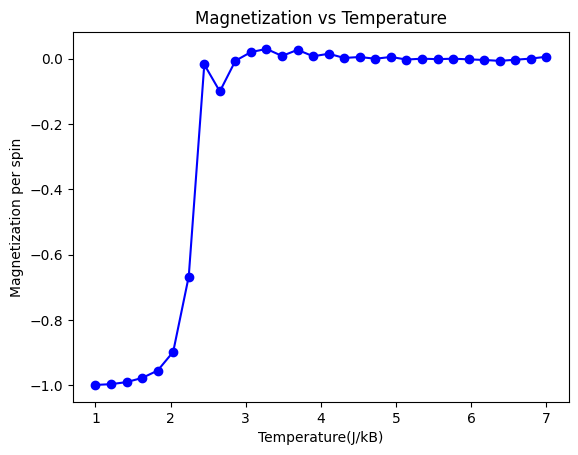
\includegraphics[scale=0.7]{magnetizationvstemp.png}
    \caption{\textbf{Average magnetization as a function of temperature}}
    \label{fig:avg_magnetization_vs_temp}
The magnetization tends to drop to zero between the temperatures $2 < T < 3$.
\end{figure}

\begin{figure}[h]
    \centering
    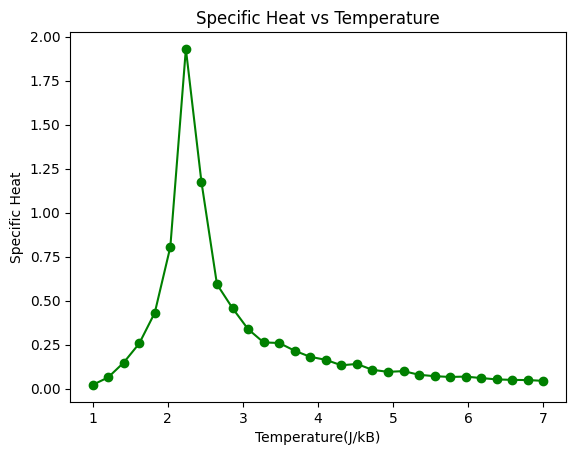
\includegraphics[scale=0.8]{spcheatvstemp.png}
    \caption{\textbf{Specific heat capacity as a function of temperature}}
    \label{fig:specific_heat_vs_temp}
A peak is observed at temperature $2 < T < 3$, and the value of specific heat approaches zero above and below these temperatures.
\end{figure}


\begin{figure}[h]
    \centering
    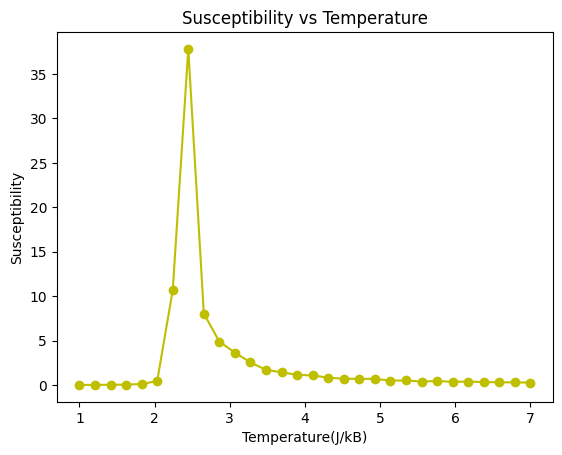
\includegraphics[scale=0.8]{susceptibilityvstemp.png}
    \caption{\textbf{Magnetic susceptibility as a function of temperature}}
    \label{fig:magnetic_susceptibility_vs_temp}
A peak is observed at temperature $2 < T < 3$, and the value of susceptibility approaches zero above and below these temperatures.
\end{figure}

\clearpage % <-- Add this command to force figures to appear before the Simulation Code section

    
\begin{figure}
    \centering
    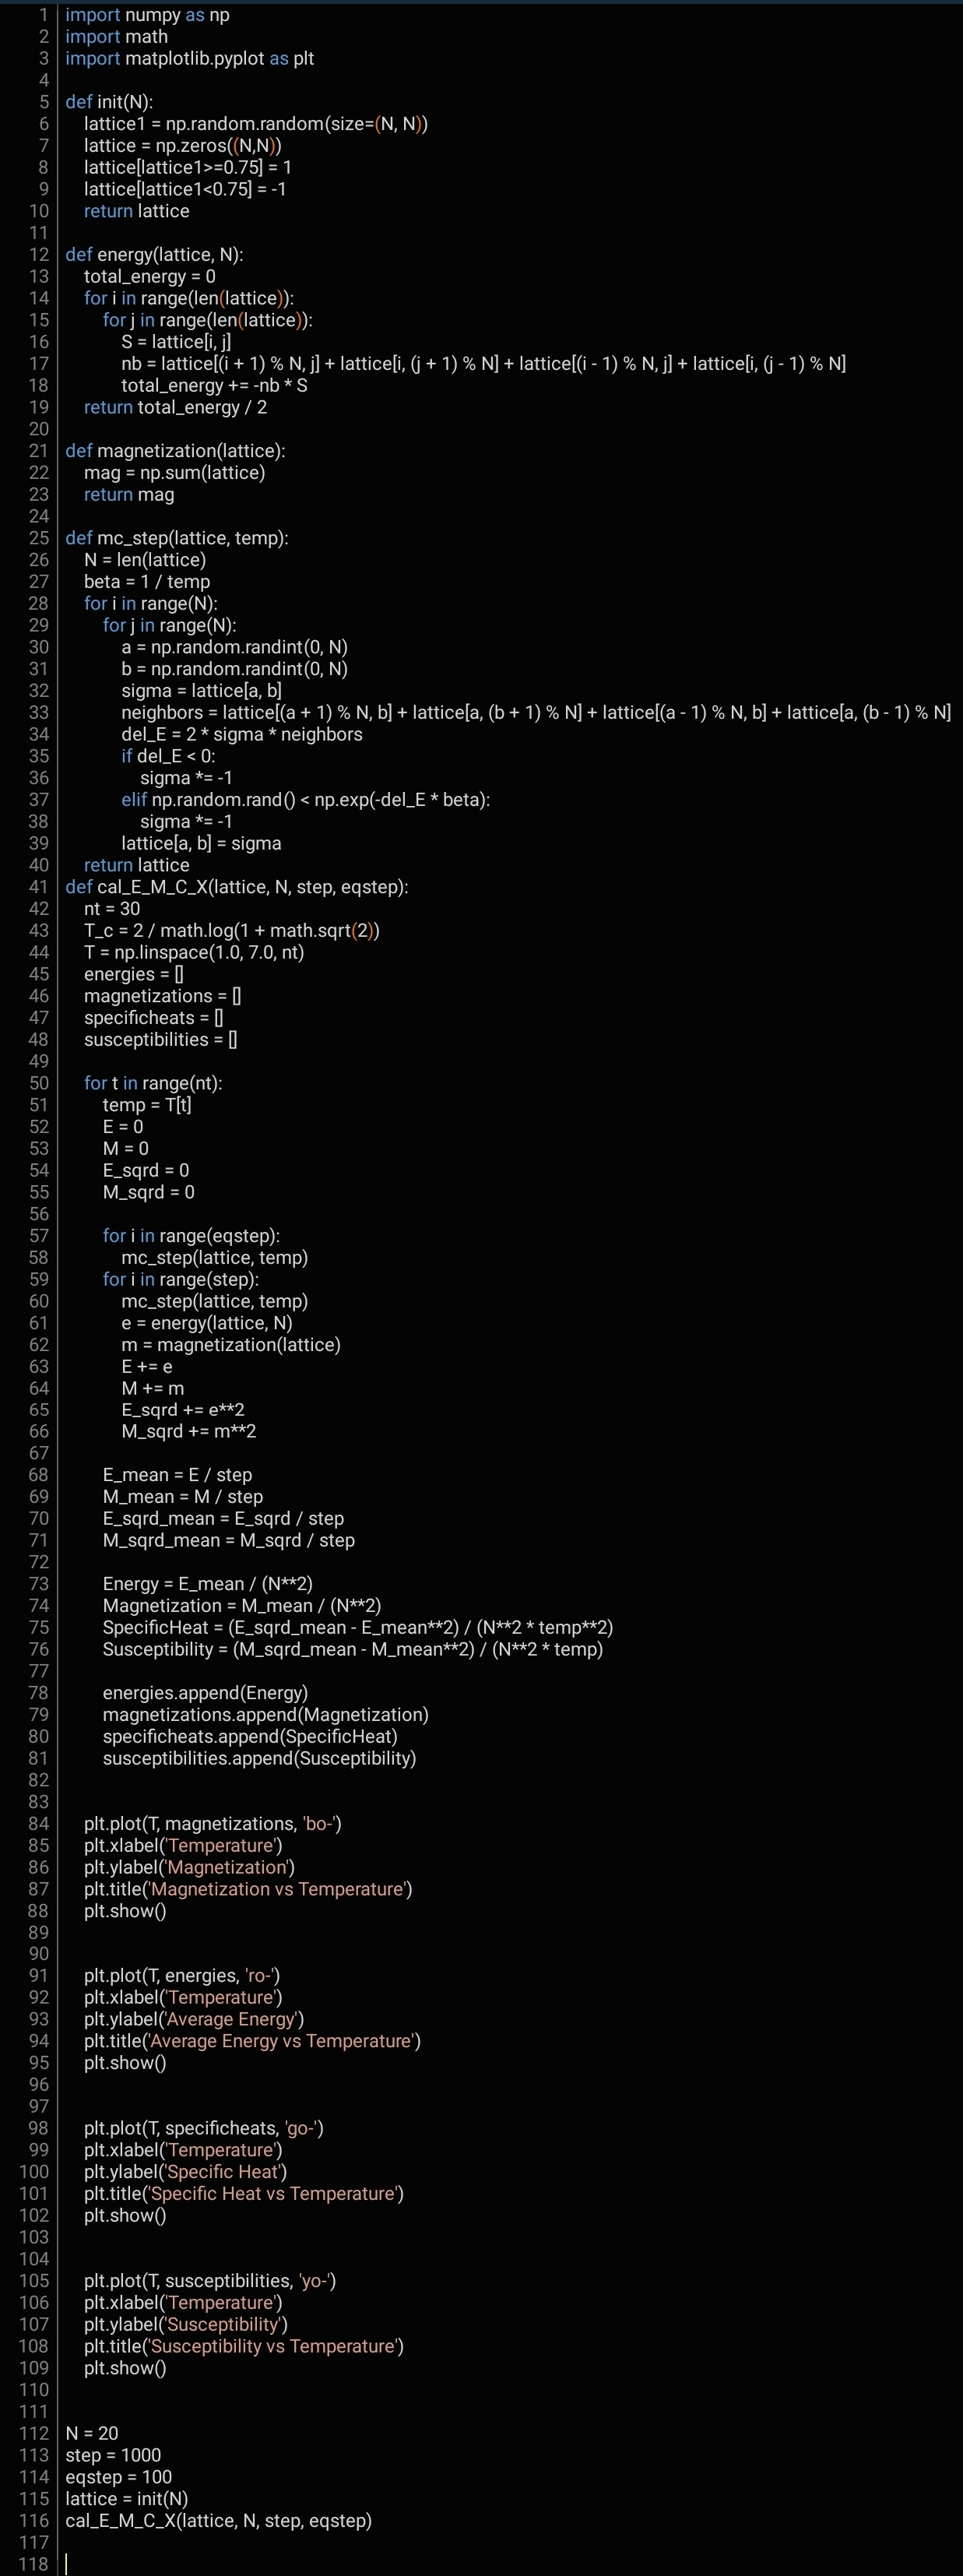
\includegraphics[width=0.5\linewidth]{IMG_20231125_233350.jpg}
    \caption{\textbf{simulation code}}
    
    
\end{figure}
 
\end{document}

